\documentclass[a4paper, 11pt]{article}
\usepackage[czech]{babel}
\usepackage{times}
\usepackage{geometry}
\usepackage[utf8]{inputenc}
\usepackage[T1]{fontenc}
\usepackage{graphicx}
\usepackage{hyperref}

\hypersetup{colorlinks = true, hypertexnames = false}

\geometry{
	a4paper,
	total={170mm, 240mm,},
	left = 20mm,
	top = 30mm,
}

\begin{document}
\begin{titlepage}
	\begin{center}
		\Huge
		\textsc{Vysoké učení technické v~Brně} \\
		\huge
		\textsc{Fakulta informačních technologií} \\
		\vspace{\stretch{0.382}}
		\LARGE
		Síťové aplikace a~správa sítí\\
		\Huge
		Přenos souboru skrz skrztý kanál
		\vspace{\stretch{0.618}}
	\end{center}
	{\Large
		\today
		\hfill
		Marek Hlávka (xhlavk09)
	}
\end{titlepage}
\tableofcontents
\newpage

\section{Zadání}
Zadáním projektu bylo vytvořit klient/server aplikaci, pomocí které bude možno přenést soubor skrz skrytý kanál, kde jsou data přenášena pomocí ICMP protokolu, resp. uvnitř ICMP Echo-Request/Response zpráv. Kvůli zabezpečení musí být soubor zašifrován pomocí šifry AES. Serverová strana aplikace pak bude ukládat soubor do složky, ve které je spuštěn.

\section{Spuštění}

\centerline{\large./secret -s <ip|hostname> -r <file> [-l]}
\begin{itemize}
\item -s <ip|hostname> : adresa nebo hostname serveru na který bude odeslaný soubor
\item -r <file> : specifikace souboru pro přenos
\item -l : program spuštěný s tímto parametrem se chová jako server, který přijímá soubory posílané od klientů
\end{itemize}
Příklad souboru s uloženými servry pro filtraci:\\
\begin{figure}[h]
%%%\includegraphics[scale=1.1]{}
\end{figure}

\section{Návrh}
Jako jazyk k implemntaci byl zvolen jazyk C. Celý program je rozdělen do dvou větších celků: 1. Strana klienta a 2. Strana serveru

\section{Argunemty}
V této části je kontrolováno spuštění programu, resp. kontrola argumentů při spuštění. K tomuto účelu je využita funkce \textit{getopt()} z knihovny \textit{getopt.h}. Jsou postupně zkontrolovány parametry, které jsou blíže popsané v sekci \textit{Spuštění}. Pokud nejsou některé požadované parametry uvedeny, program vypíše nápovědu a úspěšně se ukončí. V případě zadání parametru \textit{-l} nesjou vyžadovány další argumenty, vzhledem k tomu že server nepotřebuje cílovou ip adresu ani specifikovat souor pro přenos.

\newpage
\section{Klient}

\subsection{Načtení vstupních dat}
Po spuštění aplikace s paremetry klienta je zkontrolována daná ip addresa/hostname pomocí funkce \textit{getaddrinfo()}, která vratí informace o vstupní adrese potřebné pro další běh programu. Následně je načten samotný soubor, který je určen k přenosu. Soubor je načtený v binární formě, tudiž nezáleží na jeho připoně. Soubor je načítán najednou tudíž je jeho velikost je omezena velikosti dostupné RAM na kterém je aplikace spuštěna.

\subsection{Šifrování odesílaného paketu}
Data vstupního souboru jsou šifrována naráz, jednak kvůli jednodušší implementaci, kvůli využití místa v paketu a také kvůli zvýšené bezpečnosti, aby nebyly samostatné pakety rozšifrovatelné.

\subsection{Skládání a odesílání paketu}
%% Custom IP headers
Potřebné data k složení výsledného paketu jsou uložena do struktury \textit{icmp\_packet}, definované v souboru \textit{icmp\_packet.h}. Tato struktura slouží jako mezikrok mezi získáváním všech potřebných dat a jejich zapisováním do paketu. Následně je před odesláním tato struktura přečtena a z jejich dat jsou utvořené potřebné hlavičky a payload packetu, tzn. \textit{IP\/IPv6}, \textit{ICMP\/ICMPv6} a \textit{ICMP\_FILE} hlavičky. Hlavička \textit{ICMP\_FILE} je definovaná touto aplikací specificky pro přenos souboru pomocí icmp paketů. Výsledný paket je pak odeslán pomocí funkce \textit{sentto()} a celý tenkto krok je zopakován pro každou část dat  která vznikla rozdělením zašifrovaných dat na velikost, kterou je možné posílat po síti pomocí paketů.

\newpage
\section{Server}

\subsection{Spuštění serveru, pthread}
Po spuštění serveru jsou okamžitě vztvořeny dvě vlákna, aby mohly být přijímány současně IPv4 a IPv6 pakety. Jednak je potřeba pro každý typ paketů otevřýt soket s jinými parametry, ale také aby se program nezdržoval např. při prenosu pomocí IPv4 paketů s náhodnými ICMPv6 pakety. Po vytvoření těchto vláken program čeká na příchozí pakety, keteŕé byly zachyceny.

\subsection{Zpracování příchoyźích paketů}
Po zachycení paktu funkcí \textit{recvfrom} jsou data čtené z jednotlivých hlaviček. Při nesouhlasu důležitých informací jako např.: "icmp code", "filename" nebo "icmp type" je paket zahozen a čeká se příchod dalšího. Není tedy možné přenášet více souborů najednou, pokud není jeden přenášen pomocí IPv4 a druhý pomocí IPv6.

\subsection{Zpracování přijatých dat}
Po přijmutí všech paketů (aplikce počítá že nedochází ke ztrátám paketů), jsou jednotlivá data zkopírována dohromady, podle pořadí. Tento celek je poté rozšifrován pomocí klíče, který je zadaná přímó v programu definovaném v souboru \textit{icmp\_packet.h}.

\section{Hlavička ICMP\_FILE}
\begin{figure}[h]
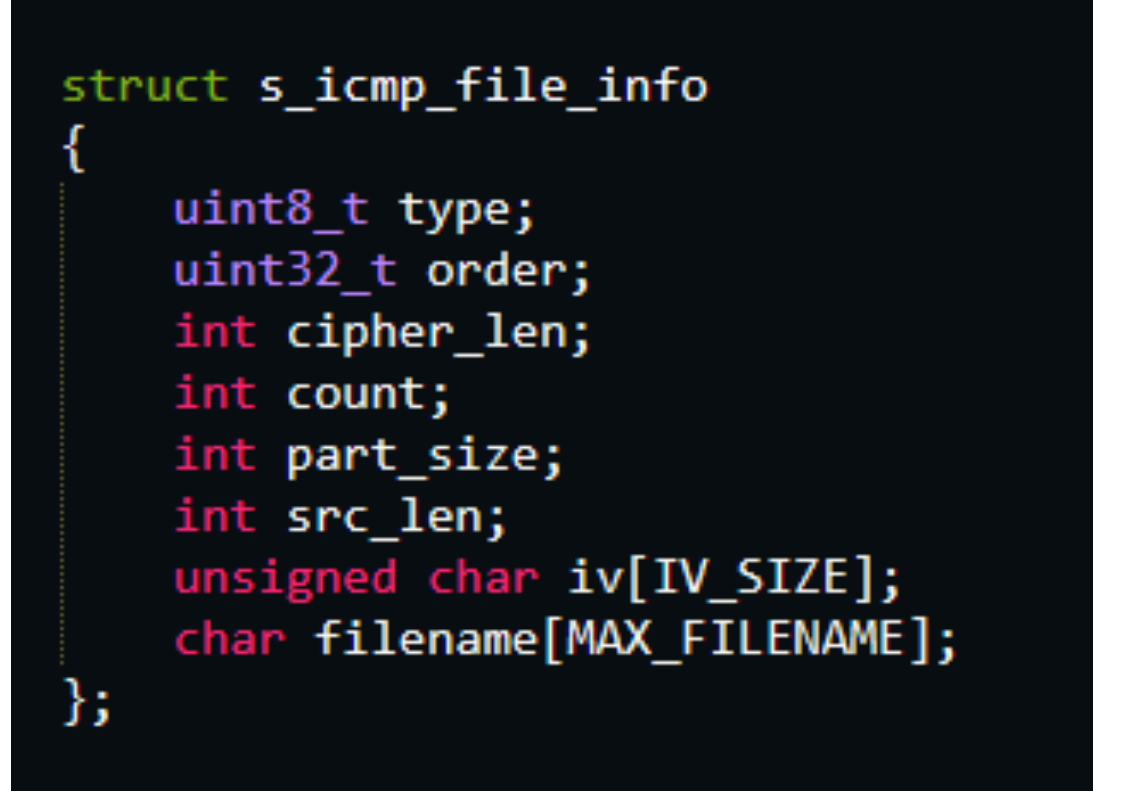
\includegraphics[scale=0.2]{img/struct.png}
\end{figure}
\begin{itemize}
\item type ....... Typ icmp\_file paketu, zejména pro případný bezpečný přenos
\item order ...... Pořadí daného paketu v celkovém přenosu
\item cipher\_len . Délka celého zašifrovaného souboru
\item count ...... Počet přenášených paketů
\item part\_size .. Velikost právě přenášených dat
\item src\_len .... Velikost původného souboru pro kontrolu po dešifrování
\item iv ......... Startovací vektor pro šifru
\item filename ... Název přenášeného souboru
\end{itemize}

\section{Šifrování}
Šifrování probíha pomocí knihovny \textit{OpenSSL}, kontrétně pomocí šifry AES. Šifrování a rozšifrování souboru pak probíha v daných funkcích v souboru \textit{aes.c}. Tato šifra je dostupná např. z \cite{aes}. Data jsou přesněji šifrována pomocí 256 bitové AES šifry v CBC módu. To vyžaduje aby klíč (key) byl dlouhý 256 bitů a startovaní vektor (iv) byl dlouhý 128 bitů.

\begin{thebibliography}{2}
\bibitem{aes}
https://wiki.openssl.org/index.php/EVP\_Symmetric\_Encryption\_and\_Decryption
\end{thebibliography}

\end{document}